\documentclass[]{article}
\usepackage[utf8]{inputenc}
\usepackage[ngerman]{babel}
\usepackage[T1]{fontenc}
\usepackage{%
	ngerman,
	ae,
	times,  %% hier kann man die Schriftart einstellen
	graphicx,
	url,
	scrlayer-scrpage,
	lastpage,
	mathtools,
	geometry,
	multicol,
	cancel,
	xcolor,
	nicematrix,
	xfrac,
	tikz,
	pgfplots,
	amsmath,
	amssymb,
	colortbl,
	centernot,
	dsfont,
	textgreek,
	icomma}
\usepackage[thinlines]{easybmat}
\usetikzlibrary{datavisualization}
\usetikzlibrary{datavisualization.formats.functions}
\usetikzlibrary{intersections}
\pgfplotsset{compat=1.17}
\newcommand{\del}[1]{\cancel{~#1~}}
\NiceMatrixOptions{ last-col,code-for-last-col = \color{blue}\scriptstyle,light-syntax}
\newlength\dlf
\newcommand\alignedhighlight[3]{
  % #1 = color
  % #2 = before alignment
  % #3 = after alignment
  &
  \begingroup
  \settowidth\dlf{$\displaystyle #2$}
  \addtolength\dlf{\fboxsep+\fboxrule}
  \hspace{-\dlf}
  \fcolorbox{#1}{#1}{$\displaystyle #2 #3$}
  \endgroup
}
\newcommand{\reference}[1]{ \text{\small{\textcolor{blue}{(#1)}}} }

\newcommand{\topic}{Mathematik 1 f"ur Informatiker}
\newcommand{\subtopic}{"Ubungsblatt 3}
\newcommand{\authors}{Nils Helming}

%Head and Footnotes
\setlength{\headheight}{2.1\baselineskip} %baselineskip = minimum distance bbetween the bottom of one line to another.
\geometry{bottom = 3cm}
\setlength{\headsep}{\baselineskip}
\ihead[\topic\hrule]{\topic\hrule}
\chead[\subtopic\\~]{\subtopic\\~}
\ohead[\authors\\~]{\authors\\~}
\ifoot[~]{~}
\cfoot[~]{~}
\ofoot[Seite \thepage~von \pageref{LastPage}]{Seite \thepage~von \pageref{LastPage}}

%Paragraph spacings
\setlength{\parindent}{0em} %em = with of an 'M'
\setlength{\parskip}{1ex} %ex = height of an 'x'


\newcommand{\V}{\lor}
\newcommand{\A}{\land}
\newcommand{\T}[1]{\overline{#1}}
\newcommand{\eq}{\Leftrightarrow}
\newcommand{\rarr}{\Rightarrow}
\newcommand{\red}[1]{\textcolor{red}{#1}}

\newcommand{\unit}[1]{\text{#1}}
\newcommand{\fracunit}[2]{\frac{\unit{#1}}{\unit{#2}}}
\newcommand{\textsq}[1]{\ensuremath{\text{#1}^2}}
\newcommand{\textpow}[2]{\ensuremath{\text{#1}^{#2}}}
\newcommand{\tdot}{\ensuremath{\cdot}}


\begin{document}

\section*{1. Aufgabe}
	\fbox{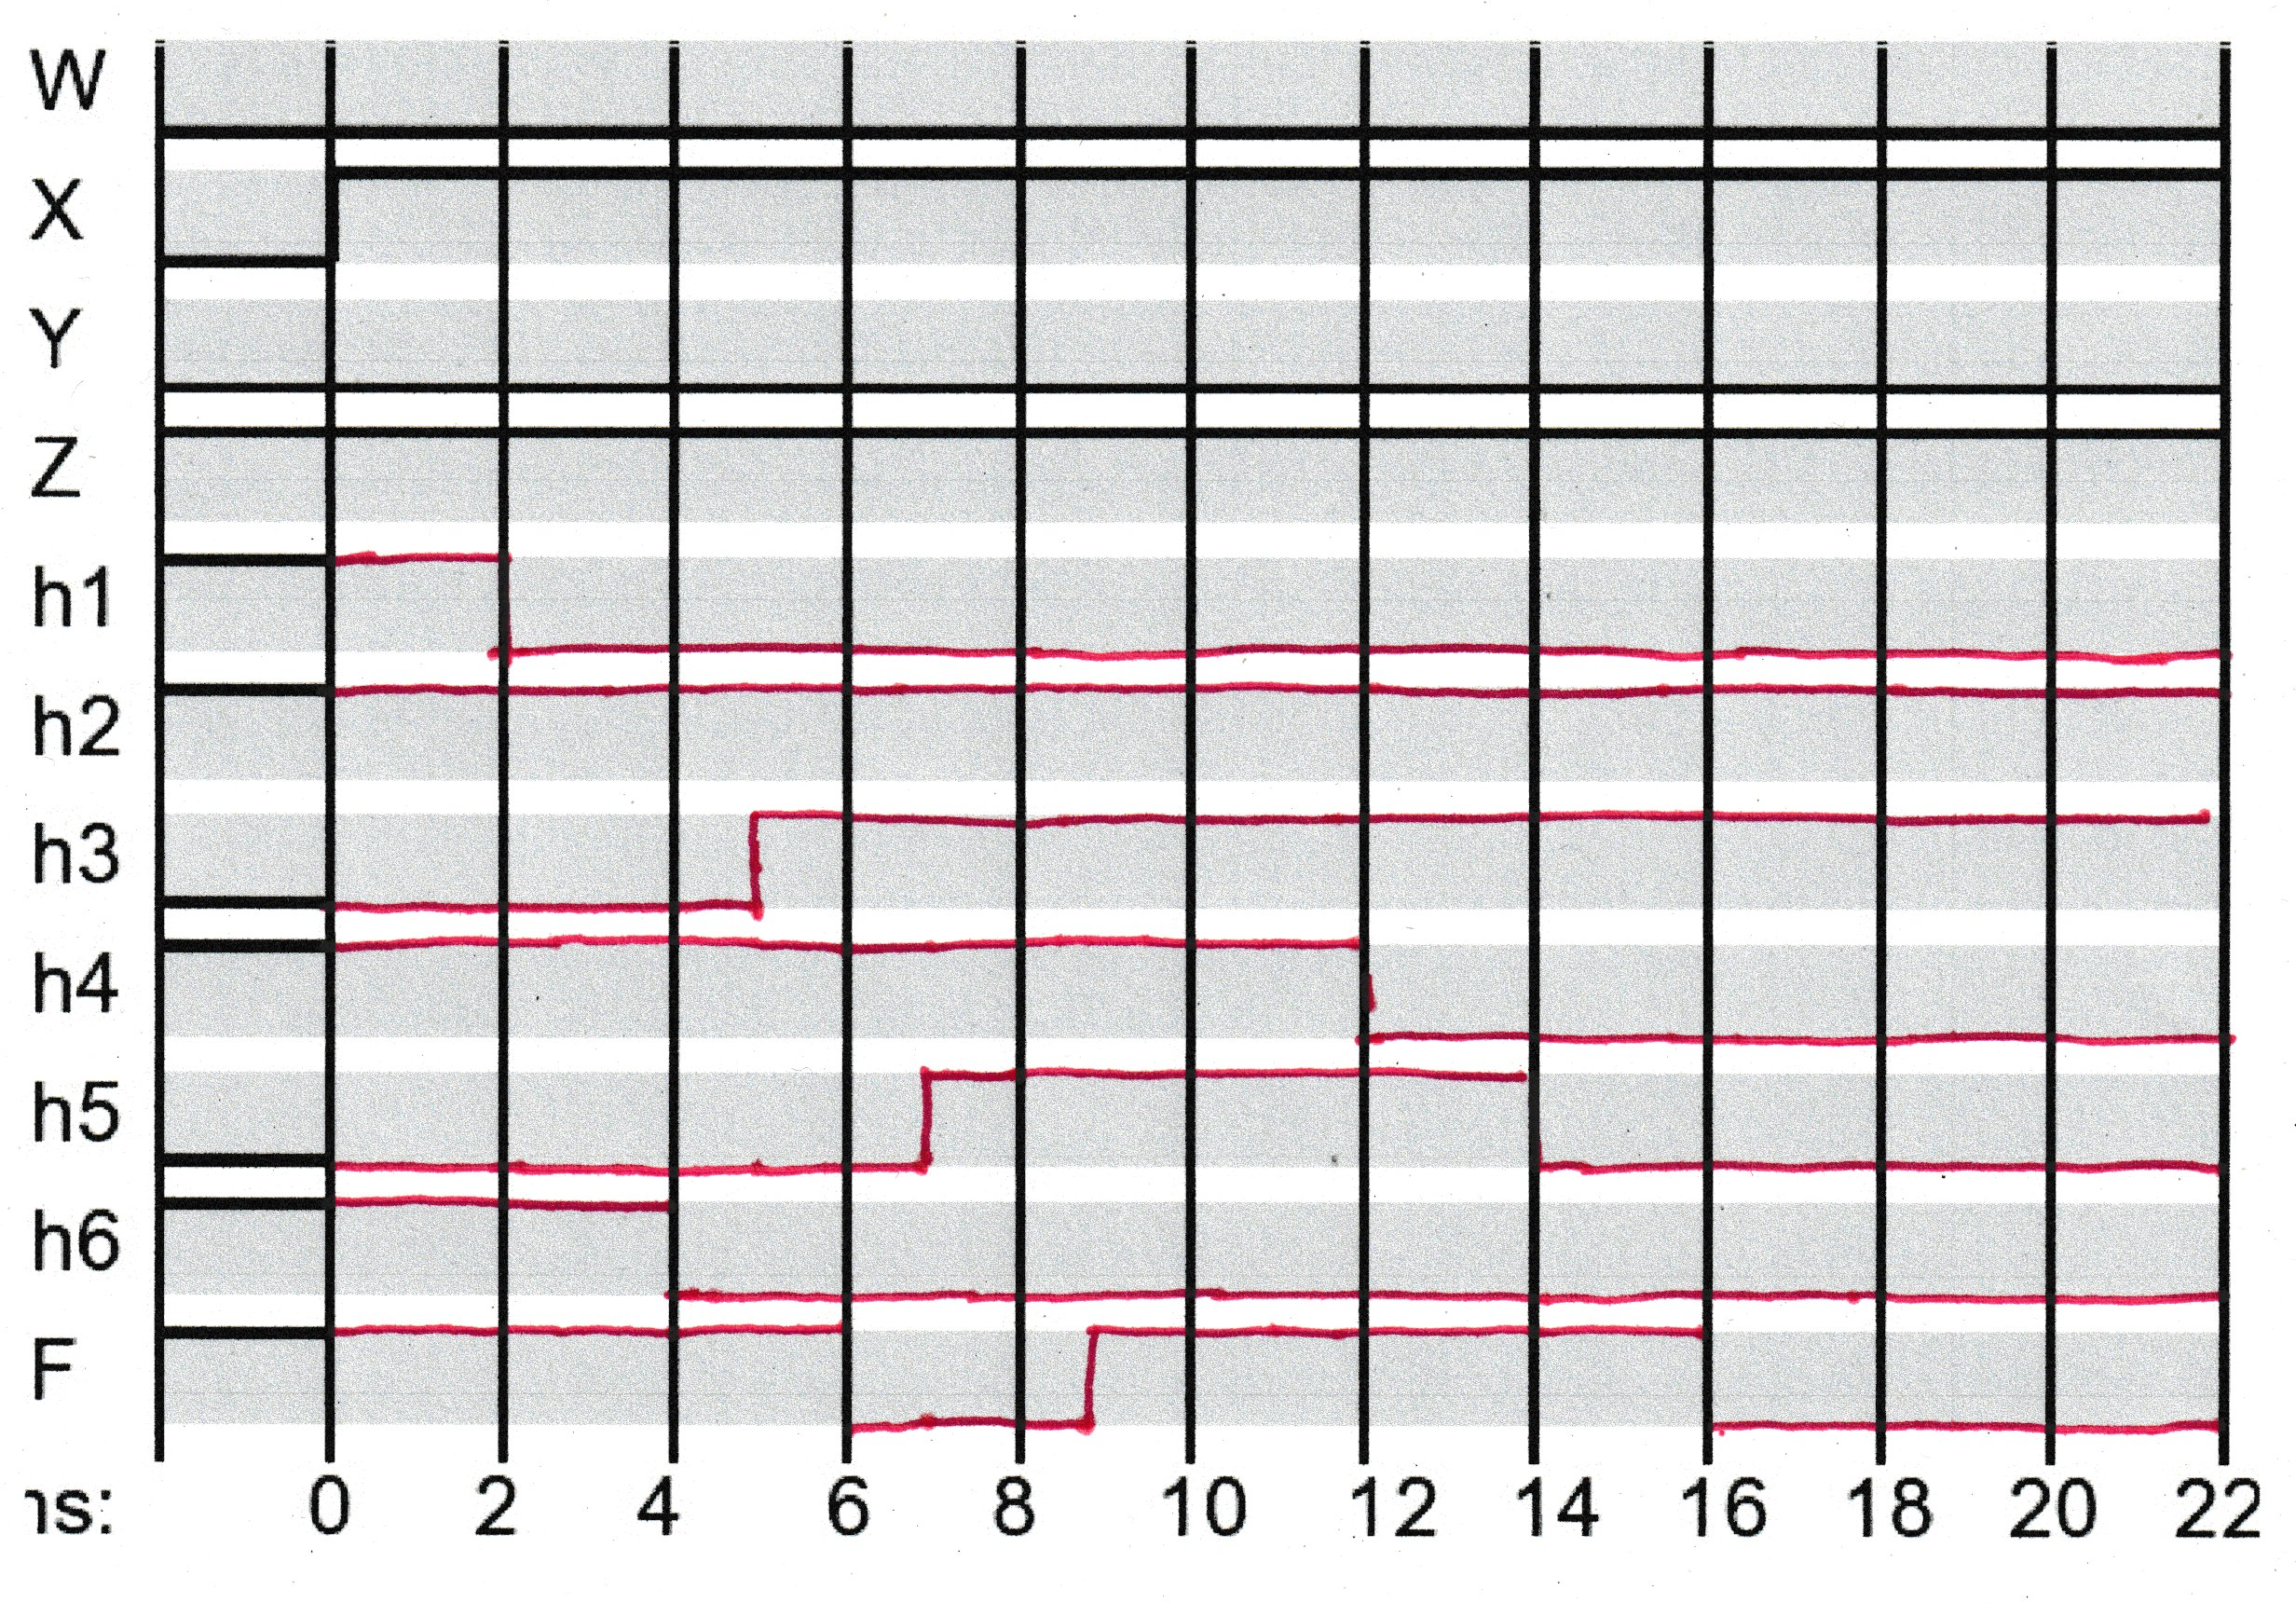
\includegraphics[scale=0.4]{Bilder/1a.png}}\par
	\fbox{\includegraphics[scale=0.4]{Bilder/1c.png}}\par
	\fbox{\includegraphics[scale=0.4]{Bilder/1d.png}}\par

\section*{2. Aufgabe}
\subsection*{a)}
\begin{align*}
	&& 8^2 - x^6 &= (2^3)^2 - x^6 &&\\
	&& &= 2^6 - x^6 &&\\
	&& &= (2^3)^2 - (x^3)^2 &&\\
	&& &= (2^3 - x^3) \cdot (2^3 + x^3) &&\\
	&& &= (2-x) \cdot (2^2- 2x + x^2) \cdot (2^3 + x^3) &&\\
	&& &\rarr p(x) = (2^2- 2x + x^2) \cdot (2^3 + x^3) &&\\
\end{align*}


\section*{3. Aufgabe}
\fbox{\includegraphics[scale=0.35]{Bilder/3.png}}\par
\begin{align*}
	&& (10n+5)^2 &= (10n)^2 + 2\cdot 10n \cdot 5 + 5^2 &&\\
	&& &= 100n^2 + 100n + 25 &&\\
	&& &= 100 \cdot n(n + 1) + 25 &&\\
\end{align*}

\section*{4. Aufgabe}
\fbox{\includegraphics[scale=0.34]{Bilder/4b.png}}\par
\fbox{\includegraphics[scale=0.34]{Bilder/4d.png}}\par

\section*{6. Aufgabe}

\subsection*{A4}
\begin{align*}
	&& A_4 &= 25r^2-40rs+16s^2+49t^2-70tq+25q^2 &&\\
	&& &= (5r-4s)^2+(7t-5q)^2 &&\\
\end{align*}
\subsection*{A5}
\fbox{\includegraphics[scale=0.35]{Bilder/6a5.png}}\par
\subsection*{A6}
\begin{align*}
	&& A_6 &= 81^2 &&\\
	&&  &= (80+1)^2 &&\\
	&&  &= 80^2 + 2 \cdot 80 \cdot 1 + 1^2 &&\\
	&&  &= 6400 + 160 + 1 &&\\
	&&  &= 6561 &&\\
\end{align*}


\subsection*{B1}
\begin{align*}
	&& B_1 &= \frac{39a^3-39a^2}{13a^2-13a} &&\\
	&& &= \frac{13a(3a^2-3a)}{13a(a-1)} &&\\
	&& &= \frac{3a^2-3a}{a-1} &&\\
	&& &= \frac{3a(a-1)}{a-1} &&\\
	&& &= 3a &&\\
\end{align*}

\subsection*{B2}
\begin{align*}
	&& B_2 &= \frac{15ab-30b^2}{5a^2b-20ab^2+20b^3} &&\\
	&& &= \frac{15ab-30b^2}{5b(a^2-4ab+4b^2)} &&\\
	&& &= \frac{15ab-30b^2}{5b(a^2-2\cdot a \cdot (2b)+(2b)^2)} &&\\
	&& &= \frac{5b(3a-6b)}{5b(a-2b)^2} &&\\
	&& &= \frac{3a-6b}{(a-2b)^2} &&\\
	&& &= \frac{3(a-2b)}{(a-2b)^2} &&\\
	&& &= \frac{3}{a-2b} &&\\
\end{align*}

\subsection*{C1}
\begin{align*}
	&& C_1 &= (-a^5)^6 \cdot (-a^6)^{-5}&&\\
	&& &= -a^{30} \cdot (-a^{-30})&&\\
	&& &= -a^{30} \cdot \frac{1}{-a^{30}}&&\\
	&& &= 1 &&\\
\end{align*}
\subsection*{C2}
\begin{align*}
	&& C_2 &= (\frac{a}{3})^2 \cdot (\frac{3}{a})^{-5}&&\\
	&& &= (\frac{a}{3})^2 \cdot (\frac{a}{3})^{5}&&\\
	&& &= (\frac{a}{3})^{2+5}&&\\
	&& &= \frac{a^7}{3^7}&&\\
	&& &= \frac{a^7}{2187}&&\\
\end{align*}

\subsection*{d1}
\begin{align*}
	&& -7 &= 3x^2+10x &&| +7\\
	&& 0 &= 3x^2+10x +7 && | :3\\
	&& 0 &= x^2+\frac{10}{3}x +\frac{7}{3} &&\\
	\text{mittels pq-formel:}&& x_{1,2} &= -\frac{\frac{10}{3}}{2} \pm \sqrt{\left(\frac{\frac{10}{3}}{2}\right)^2 - \frac{7}{3}} &&\\
	&& &= -\frac{10}{6} \pm \sqrt{\left(\frac{10}{6}\right)^2 - \frac{7}{3}} &&\\
	&& &= -\frac{10}{6} \pm \sqrt{\frac{100}{36} - \frac{7}{3}} &&\\
	&& &= -\frac{10}{6} \pm \sqrt{\frac{100}{36} - \frac{84}{36}} &&\\
	&& &= -\frac{10}{6} \pm \sqrt{\frac{16}{36}} &&\\
	&& &= -\frac{10}{6} \pm \frac{\sqrt{16}}{\sqrt{36}} &&\\
	&& &= -\frac{10}{6} \pm \frac{4}{6} &&\\
	\\
	&& \rarr \mathbb{L} &= \left\{-\frac{10}{6} - \frac{4}{6}, -\frac{10}{6} + \frac{4}{6}\right\} &&\\
	&& &= \left\{-\frac{7}{3}, -1\right\} &&\\
\end{align*}

\subsection*{d2}
\begin{align*}
	&& 2x-3 &= 2x^2 && \\
	&&\eq 0 &= 2x^2 -2x +3 && |:2\\
	&&\eq 0 &= x^2 -x +\frac{3}{2} &&\\
	&& &\rarr \left(\frac{p}{2}\right)^2 - q < 0 \text{ mit } p=-1 \text{ und } q = \frac{3}{2} &&\\
	&& &\rarr \mathbb{L} = \emptyset  \text{ da die Diskriminante unter $0$ liegt.}&&\\
\end{align*}
\subsection*{d5}
\begin{align*}
	&& 0 &= (x-2)(x-5)+2 && \\
	&& &= (x^2-5x-2x+10)+2 && \\
	&& &= x^2-7x+12 && \\
	\text{mittels pq-formel:}&& x_{1,2} &= -\frac{-7}{2} \pm \sqrt{\left(\frac{-7}{2}\right)^2 - 12} &&\\
	&& &= \frac{7}{2} \pm \sqrt{\left(\frac{49}{4}\right) - 12} &&\\
	&& &= \frac{7}{2} \pm \sqrt{\frac{49}{4} - \frac{48}{4}} &&\\
	&& &= \frac{7}{2} \pm \sqrt{\frac{1}{4}} &&\\
	&& &= \frac{7}{2} \pm \frac{1}{2} &&\\
	&& \rarr \mathbb{L} &= \left\{\frac{6}{2}, \frac{8}{2}\right\} &&\\
	&& &= \{3, 4\} &&\\
\end{align*}


\end{document}